
% FILE: figures/thresholds_taxonomy.tex
% Taxonomy of thresholds

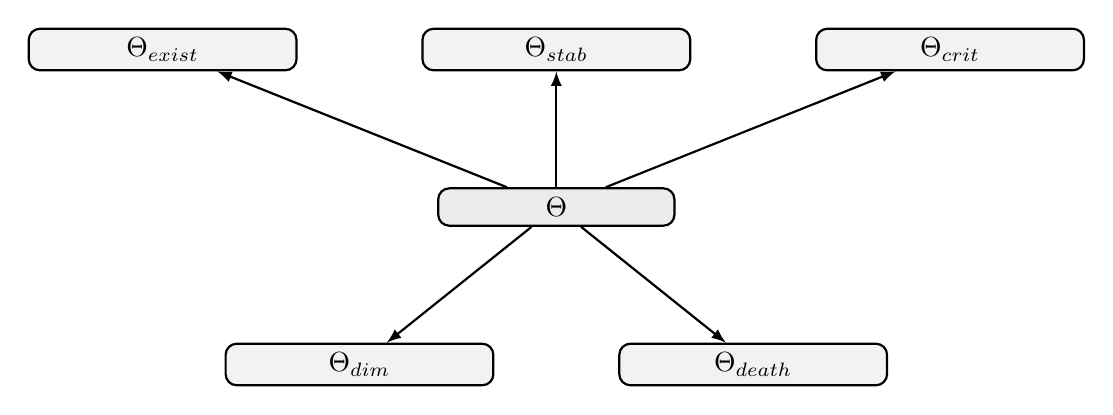
\begin{tikzpicture}[>=latex,thick]
  % Central node
  \node[draw, rounded corners, fill=gray!15, minimum width=3cm] (Theta) at (0,0) {$\Theta$};

  % Children
  \node[draw, rounded corners, fill=gray!10, minimum width=3.4cm] (exist) at (-5, 2) {$\Theta_{\text{exist}}$};
  \node[draw, rounded corners, fill=gray!10, minimum width=3.4cm] (stab)  at ( 0, 2) {$\Theta_{\text{stab}}$};
  \node[draw, rounded corners, fill=gray!10, minimum width=3.4cm] (crit)  at ( 5, 2) {$\Theta_{\text{crit}}$};

  \node[draw, rounded corners, fill=gray!10, minimum width=3.4cm] (dim)   at (-2.5,-2) {$\Theta_{\text{dim}}$};
  \node[draw, rounded corners, fill=gray!10, minimum width=3.4cm] (death) at ( 2.5,-2) {$\Theta_{\text{death}}$};

  % Arrows
  \draw[->] (Theta) -- (exist);
  \draw[->] (Theta) -- (stab);
  \draw[->] (Theta) -- (crit);
  \draw[->] (Theta) -- (dim);
  \draw[->] (Theta) -- (death);
\end{tikzpicture}
